\documentclass[main.tex]{subfiles}
\begin{document}
\begin{enumerate}
% -----------------------------------------------------
% Question and Answer 1
% -----------------------------------------------------
\item{\textbf{Signum phase mask.} The imaging system shown in Figure \ref{fig:f1} is illuminated by an on-axis plane wave at wavelength $\lambda=\SI{1}{\mu \meter}$. }

\begin{figure}
\centering\fbox{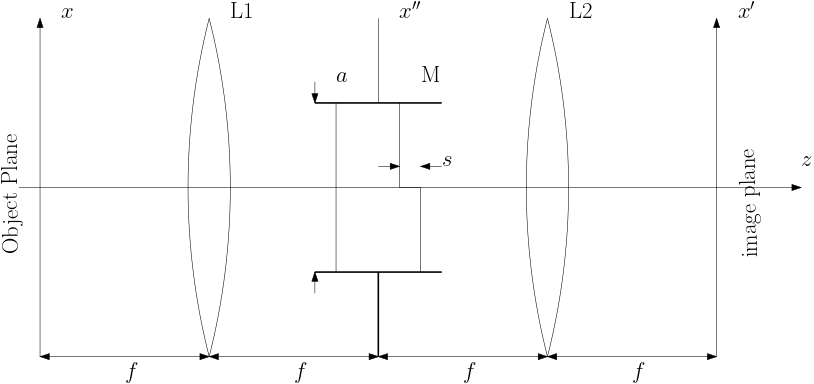
\includegraphics[height=2.0in]{figures/final/1_a_imaging_system.png}}
\caption{Lenses L1, L2 are identical with sufficiently large aperture and focal length $f=\SI{10}{c\metre}$. The pupil mask M has aperture $a=\SI{1}{c\metre}$. Inside the aperture there is a piece of glass of refractive index $n=1.5$. The glass has been partially etched to form a step of height $s=\SI{1}{\mu \metre}$, and the step is precisely aligned with the optical axis, as shown.}
\label{fig:f1}
\end{figure}

\begin{enumerate}
\item{Sketch the amplitude transfer function (AFT) of this optical system.}\\

The phase shift induced by the mask is defined in Equation \ref{eq:fa11}.

\begin{equation}\label{eq:fa11}
\varphi = \frac{2\pi}{\lambda}s(n-1) = \frac{2\pi}{\SI{1}{\mu \metre}}(\SI{1}{\mu \metre})(0.5)=\pi
\end{equation}

Hence, the pupil function can be written in Equation \ref{eq:fa12}.

\begin{equation}\label{eq:fa12}
P(x^{\prime \prime}) = \text{rect}(\frac{x^{\prime \prime} - a/4}{a/2}) + \text{rect}(\frac{x^{\prime \prime} + a/4}{a/2}) e^{i\pi}
\end{equation}

AFT is a scaled pupil function, which is found in Equation \ref{eq:fa13}.

\begin{equation}\label{eq:fa13}
H(u) = P(\lambda f u) = \text{rect}(\frac{\lambda f u - a/4}{a/2}) + \text{rect}(\frac{\lambda f u + a/4}{a/2}) e^{i\pi}
\end{equation}

A Sketch of the ATF magnitude and phase angle shown in Figure \ref{fig:f2}.

\begin{figure}
\centering\fbox{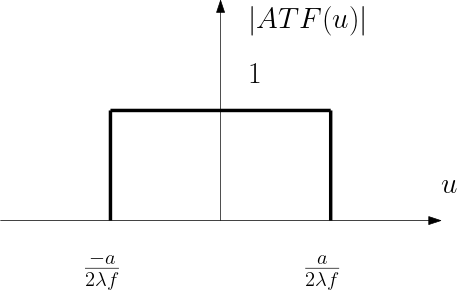
\includegraphics[width=2.0in]{figures/final/1_b_atf_magnitude.png}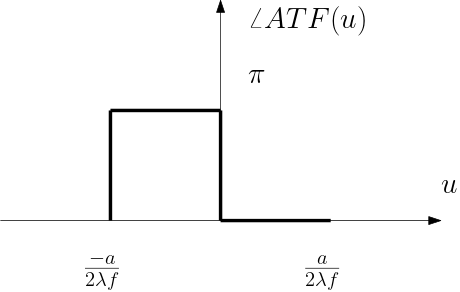
\includegraphics[width=2.0in]{figures/final/1_c_atf_phase.png}}
\caption{Amplitude Transfer Function magnitude and phase angle where $a/(2\lambda f) = \frac{1}{20}\mu \text{m} $ }
\label{fig:f2}
\end{figure}

\item{A thin transparency with amplitude transmission function}
$$g_t(x)=\cos \left( 2\pi \frac{x}{\SI{20}{\mu \metre} } \right)$$ 
is placed at the object plane. Sketch the magnitude and phase of the transparency $g_t(x)$.\\

A Sketch of the Transparency magnitude and phase angle shown in Figure \ref{fig:f3}.

\begin{figure}
\centering\fbox{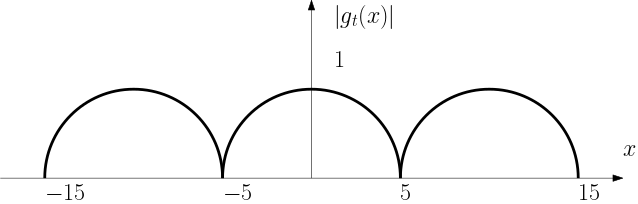
\includegraphics[width=2.0in]{figures/final/1_d_transparency_magnitude.png}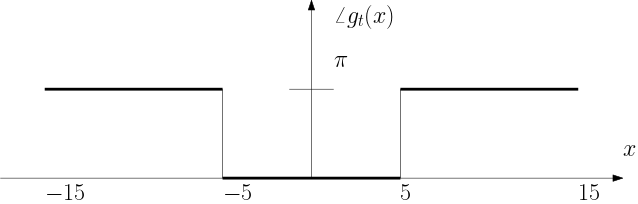
\includegraphics[width=2.0in]{figures/final/1_e_transparency_phase.png}}
\caption{Transparency magnitude and phase angle}
\label{fig:f3}
\end{figure}

\item{With the transparency $g_t(x)$ in place at the object plane, the system is illuminated with a plane wave on-axis. What is the optical field at the image plane?}\\

The optical field at the image plane can be obtained from two ways: 1) direct forward computation or 2) frequency analysis. [1] direct forward computation: The incident field to the Fourier plane is defined in Equation \ref{eq:fa14}.


\begin{equation}\label{eq:fa14}
\begin{aligned} 
\mathfrak{F}\left[\cos \left(2 \pi \frac{x}{\Lambda}\right)\right]_{\frac{x^{\prime \prime}}{\lambda f}} =
& \frac{1}{2} \delta\left(\frac{x^{\prime \prime}}{\lambda f}-\frac{1}{\Lambda}\right)+\frac{1}{2} \delta\left(\frac{x^{\prime \prime}}{\lambda f}+\frac{1}{\Lambda}\right)\\
                                                                                                       =& \frac{1}{2} \delta\left(x^{\prime \prime}-5 \mathrm{mm}\right)+\frac{1}{2} \delta\left(x^{\prime \prime}+5 \mathrm{mm}\right)
\end{aligned}
\end{equation}

Since the width of the pupil is \SI{10}{m\metre}, both delta functions pass through the pupil with a phase delay. The field immediately after the phase mask is defined in Equation \ref{eq:fa15}.

\begin{equation}\label{eq:fa15}
\frac{1}{2} \delta\left(x^{\prime \prime}-5\right)+e^{i \pi} \frac{1}{2} \delta\left(x^{\prime \prime}+5\right) =\frac{1}{2} \delta\left(x^{\prime \prime}-5\right)-\frac{1}{2} \delta\left(x^{\prime \prime}+5\right)
\end{equation}

The field at the image plane is defined in Equation \ref{eq:fa16}.

\begin{equation}\label{eq:fa16}
\begin{aligned} 
\mathfrak{F}\left[\frac{1}{2} \delta\left(x^{\prime \prime}-5\right)-\frac{1}{2} \delta\left(x^{\prime \prime}+5\right)\right]_{\frac{x^{\prime}}{\lambda f}}\\
=i \mathfrak{F}\left[\frac{1}{2 i} \delta\left(x^{\prime \prime}-5\right)-\frac{1}{2 i} \delta\left(x^{\prime \prime}+5\right)\right]_{\frac{x^{\prime}}{\lambda f}} \\
=i \sin \left(2 \pi \frac{1}{5} \frac{x^{\prime}}{\lambda f}\right)=i \sin \left(2 \pi \frac{x^{\prime}}{20 \mu m}\right) 
\end{aligned}
\end{equation}

[2] frequency analysis: The Fourier transform of the output field is a multiplication of the Fourier transform of the input field and the ATF. Since the Fourier transform of the input signal is $\frac{1}{2} \delta\left(u-\frac{1}{20 \mu \mathrm{m}}\right)+\frac{1}{2} \delta\left(u+\frac{1}{20 \mu \mathrm{m}}\right)$, the FT of the output field is defined in Equation \ref{eq:fa17}.

\begin{equation}\label{eq:fa17}
\frac{1}{2} \delta\left(u-\frac{1}{20 \mu m}\right)-\frac{1}{2} \delta\left(u+\frac{1}{20 \mu m}\right)
\end{equation}

Therefore the output field is $i \sin \left(2 \pi \frac{x^{\prime}}{20 \mu \mathrm{m}}\right)$.

\item{With the same transparency $g_t(x)$ in place at the object plane, the system is illuminated with a plane wave off-axis, propagating at an angle of +0.1rad with respect to the optical axis. What is the optical field at the image plane?}\\

Similarly we can analyze with either 1) direct forward computation or 2) frequency analysis. [1] If the incident wave is tilted, then one of the two delta functions at the Fourier plane is blocked by the pupil. The other delta function still gets phase delay and propagates to the image plane. The field immediately after the grating is defined in Equation \ref{eq:fa18}.

\begin{equation}\label{eq:fa18}
\exp \left\{i \frac{2 \pi}{\lambda} \theta x\right\} \cos \left(2 \pi \frac{x}{20 \mu m}\right)
\end{equation}

Then the field incident to the Fourier plane is defined in Equation \ref{eq:fa19}.

\begin{equation}\label{eq:fa19}
\begin{aligned} 
\mathfrak{F}\left[\exp \left\{i \frac{2 \pi}{\lambda} \theta x\right\} \cos \left(2 \pi \frac{x}{20 \mu \mathrm{m}}\right)\right]_{\frac{x^{\prime \prime}}{\lambda f}}\\
=\delta\left(\frac{x^{\prime \prime}}{\lambda f}-\frac{\theta}{\lambda}\right) \otimes\left\{\frac{1}{2} \delta\left(\frac{x^{\prime \prime}}{\lambda f}-\frac{1}{\Lambda}\right)+\frac{1}{2} \delta\left(\frac{x^{\prime \prime}}{\lambda f}+\frac{1}{\Lambda}\right)\right\} \\ 
= \frac{1}{2} \delta\left(x^{\prime \prime}-\theta f-\frac{\lambda f}{\Lambda}\right)+\frac{1}{2} \delta\left(x^{\prime \prime}-\theta f+\frac{\lambda f}{\Lambda}\right) \\
=\frac{1}{2} \delta\left(x^{\prime \prime}-10 \mathrm{mm}-5 \mathrm{mm}\right)+\frac{1}{2} \delta\left(x^{\prime \prime}-10 \mathrm{mm}+5 \mathrm{mm}\right)
\end{aligned}
\end{equation}

Where the second delta function does not get phase delay now. The field at the output plane is defined in Equation \ref{eq:fa110}.

\begin{equation}\label{eq:fa110}
\begin{aligned} 
\mathfrak{F}\left[\frac{1}{2} \delta\left(x^{\prime \prime}-5 \mathrm{mm}\right)\right]_{\frac{x^{\prime}}{\lambda f}}\\
=\frac{1}{2} \exp \left\{-i 2 \pi \frac{x^{\prime}}{\lambda f}(5 \mathrm{mm})\right\}\\
=\frac{1}{2} \exp \left\{i \frac{2 \pi}{\lambda}(-0.05) x^{\prime}\right\}
\end{aligned}
\end{equation}

Thus, the output field is a tilted plane wave with an angle of $-0.05$ rad. The factor of $\frac{1}{2}$ indicates that the amplitude of the output field is half of the amplitude of the input field.\\ 

[2] The spatial frequency of the tilted plane wave is $u = \frac{\theta}{\lambda} = \SI{0,1}{\mu \metre^{-1}}$. Then, the field immediately after the grating is defined in Equation \ref{eq:fa111}.

\begin{equation}\label{eq:fa111}
\frac{1}{2} \delta\left(u-\frac{1}{10 \mu m}-\frac{1}{20 \mu m}\right)+\frac{1}{2} \delta\left(u-\frac{1}{10 \mu m}+\frac{1}{20 \mu m}\right)
\end{equation}

Then, the FT of the output field is defined in \ref{eq:fa112}.

\begin{equation}\label{eq:fa112}
\frac{1}{2} \delta\left(u-\frac{1}{20 \mu m}\right)
\end{equation}

Therefore the output field is defined in Equation \ref{eq:fa113}.

\begin{equation}\label{eq:fa113}
\frac{1}{2} \exp \left\{-i 2 \pi\left(\frac{1}{20} x^{\prime}\right)\right\}=\frac{1}{2} \exp \left\{i \frac{2 \pi}{\lambda}(-0.05) x^{\prime}\right\}
\end{equation}

\item{Suggest an intuitive description of the system's operation under spatially coherent, on-axis plane wave illumination (as in question c)}.\\

At the  Fourier plane, a signum function with a $\pi$ phase shift is multiplied. It is equivalent to the Hilbert transform. Note that the Hilbert transform converts $\cos$ to $\sin$ and vise versa.

\end{enumerate}

% -----------------------------------------------------
% Question  and Answer 2
% -----------------------------------------------------
\item{\textbf{Grating with tilted plane wave illumination} Consider a sinusoidal phase grating of the surface relief type with complex amplitude transmission function defined in Equation \ref{eq:fq21}}.

\begin{equation}\label{eq:fq21}
g_{\mathrm{t}}(x)=\exp \left\{i \frac{m}{2} \sin \left(2 \pi \frac{x}{\Lambda}\right)\right\}
\end{equation}

The grating is placed at the plane $z=0$ and illuminated by an off-axis plane wave defined in Equation \ref{eq:fq22} propagating at angle $\theta << 1$ with respect to the optical axis $z$.

\begin{equation}\label{eq:fq22}
\begin{aligned} 
g_{-}(x, z=0)&=\left.\exp \left\{i 2 \pi \frac{x}{\lambda} \sin \theta+i 2 \pi \frac{z}{\lambda} \cos \theta\right\}\right|_{z=0} \\
&\approx \exp \left\{i 2 \pi \frac{\theta x}{\lambda}\right\}
\end{aligned} 
\end{equation}

\begin{enumerate}
\item{Describe, in as much detail as possible, the Fresnel diffraction pattern $g_+(x,z=0)$.} \\

In this problem, one dimensional geometry along the $x$-axis is considered. The Fresnel diffraction pattern, the field just behind the grating illuminated by the plane wave, is defined in Equation \ref{eq:fa21}.

\begin{equation}\label{eq:fa21}
\begin{aligned} 
g_{+}(x, z=0)&=g_{t}(x) g_{-}(x, z=0)\\
&=\exp \left\{i \frac{m}{2} \sin \left(2 \pi \frac{x}{\Lambda}\right)\right\} \exp \left\{i \frac{2 \pi}{\lambda} \theta x\right\}
\end{aligned} 
\end{equation}

Note that the transmission function can be expanded as shown in Equation \ref{eq:fa22}.

\begin{equation}\label{eq:fa22}
\begin{aligned} 
g_{t}(x)&=\exp \left\{i \frac{m}{2} \sin \left(2 \pi \frac{x}{\Lambda}\right)\right\}\\
&=\sum_{q=-\infty}^{\infty} J_{q}\left(\frac{m}{2}\right) \exp \left\{i q \frac{2 \pi}{\Lambda} x\right\}
\end{aligned} 
\end{equation}

Using Equation \ref{eq:fa22}, we can rewrite Equation \ref{eq:fa21} as Equation \ref{eq:fa23}.

\begin{equation}\label{eq:fa23}
g_{+}(x, z=0)=\sum_{q=-\infty}^{\infty} J_{q}\left(\frac{m}{2}\right) \exp \left\{i \frac{2 \pi}{\lambda}\left(\theta+\frac{q \lambda}{\Lambda}\right) x\right\}
\end{equation}

Since $\exp \left\{i \frac{2 \pi}{\lambda}\left(\theta+\frac{q \lambda}{\Lambda}\right) x\right\}$ represents a tilted plane wave whose propagation angle is $\theta + q\lambda / \Lambda$, Equation \ref{eq:fa23} implies that the transmitted field just behind the grating is consisted of a infinite number of plane waves, where $q$ denotes diffraction order and the amplitude of the diffraction order $q$ is $J_q(m/2)$. The propagation direction of the zero-order is identical as one of the incident tilted plane wave.\\

\item{Describe, in as much detail as possible, the Fraunhofer diffraction pattern.}\\

The field behind the grating is identical to Equation \ref{eq:fa21}. When the observation plane is in the far-zone, the Fraunhofer diffraction pattern is defined as Equation \ref{eq:fa24}.

\begin{equation}\label{eq:fa24}
g\left(x^{\prime}, z\right)=\int g_{+}(x, z=0) \exp \left\{-i \frac{2 \pi}{\lambda z}\left(x^{\prime} x\right)\right\} \mathrm{d} x
\end{equation}

Note that we neglected the scaling factor and phase term because the scaling factor changes overall magnitude of diffraction pattern and the phase term does not contribute to intensity. Substituting Equation \ref{eq:fa22} into Equation \ref{eq:fa24}, we obtain the field distribution of the Fraunhofer diffraction in Equation \ref{eq:fa25}.

\begin{equation}\label{eq:fa25}
\begin{aligned} 
g\left(x^{\prime}, z\right)&= \int\left[\sum_{q=-\infty}^{\infty} J_{q}\left(\frac{m}{2}\right) \exp \left\{i \frac{2 \pi}{\lambda}\left(\theta+\frac{q \lambda}{\Lambda}\right)\right\}\right] \exp \left\{-i \frac{2 \pi}{\lambda z}\left(x x^{\prime}\right)\right\} \mathrm{d} x \\
&=\sum_{q=-\infty}^{\infty} J_{q}\left(\frac{m}{2}\right)\left[\int \exp \left\{i 2 \pi\left(\frac{q}{\Lambda}+\frac{\theta}{\lambda}\right) x\right\} \exp \left\{-i 2 \pi \frac{x^{\prime}}{\lambda z} x\right\} \mathrm{d} x\right] \\
&=\sum_{q=-\infty}^{\infty} J_{q}\left(\frac{m}{2}\right) \delta\left(\frac{x^{\prime}}{\lambda z}-\left[\frac{q}{\Lambda}+\frac{\theta}{\lambda}\right]\right)
\end{aligned} 
\end{equation}

\begin{figure}
\centering\fbox{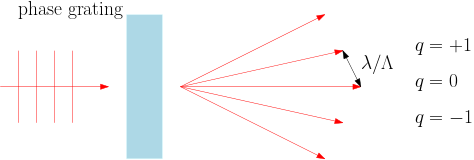
\includegraphics[width=2.0in]{figures/final/2_a_diffraction.png}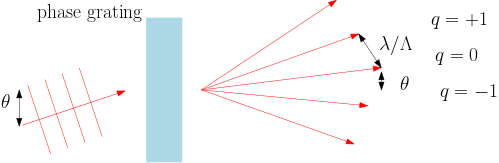
\includegraphics[width=2.0in]{figures/final/2_b_diffraction_rotate.png}}
\caption{The whole diffraction pattern rotates by $\theta$ as the incident plane wave rotates}
\label{fig:fa21}
\end{figure}

The intensity of the Fraunhofer diffraction pattern is defined in Equation \ref{eq:fa26}.

\begin{equation}\label{eq:fa26}
\begin{aligned} 
I\left(x^{\prime}, z\right)&= \left|g\left(x^{\prime}, z\right)\right|^{2}\\
&=\sum_{q=-\infty}^{\infty} J_{q}^{2}\left(\frac{m}{2}\right) \delta\left(\frac{x^{\prime}}{\lambda z}-\left[\frac{q}{\Lambda}+\frac{\theta}{\lambda}\right]\right)
\end{aligned} 
\end{equation}

In the far-region, we should observe a infinite number of diffraction orders. The in-tensity of the diffraction order is proportional to $J_q^2(m/2)$ and the offset between two neighboring diffraction orders is $(\lambda z)/\Lambda$. The zeroth order is located at $x^{\prime}=z\theta$.

\item{Compare with the on-axis illuminated phase grating that we analyzed in class.}\\

In both cases (Fresnel and Fraunhofer diffraction), the diffraction patterns of the grating probed by a on-axis and tilted plane waves are identical except the angular shift by the incident angle $\theta$, as shown in Figure \ref{fig:fa21}.


\end{enumerate}
% -----------------------------------------------------
% Question 3 Answer in Hw 5
% -----------------------------------------------------

% -----------------------------------------------------
% Question 4 Answer in Hw 5
% -----------------------------------------------------

% -----------------------------------------------------
% Question 5 Answer in Hw 5
% -----------------------------------------------------
\end{enumerate}


\end{document}